%----------------------------------------------------------------------------------------
%	PACKAGES AND OTHER DOCUMENT CONFIGURATIONS
%----------------------------------------------------------------------------------------

\documentclass[12pt]{article}
\usepackage{polski}
\usepackage[polish]{babel}
\usepackage[utf8]{inputenc}
\usepackage{datetime}
\usepackage{graphicx}
\usepackage{tikz}
\usepackage{amsmath}
\usepackage{multirow}
\usepackage{tabularx}
\usepackage{geometry}
\usepackage{subcaption}
\usepackage{epstopdf}
\usepackage{indentfirst}

\geometry{
 	a4paper, 
 	left    = 20mm,
 	right	  = 20mm,
 	top     = 20mm,
 	bottom  = 20mm,
}
 
%----------------------------------------------------------------------------------------
 
%----------------------------------------------------------------------------------------
% DATES
%----------------------------------------------------------------------------------------

\renewcommand{\dateseparator}{.}
\newdate{exercise_date}{15}{12}{2016}


% dodatkowe typy kolumn tabel

% flush left fixed width:
\newcolumntype{L}[1]{>{\raggedright\arraybackslash}p{#1}}

% center fixed width:
\newcolumntype{C}[1]{>{\centering\arraybackslash}p{#1}}

% flush right fixed width:
\newcolumntype{R}[1]{>{\raggedleft\arraybackslash}p{#1}}

%----------------------------------------------------------------------------------------

%----------------------------------------------------------------------------------------
% TIKZ PACKAGES
%----------------------------------------------------------------------------------------

\usetikzlibrary{arrows}

%----------------------------------------------------------------------------------------

\begin{document}
 
\begin{titlepage}

\newcommand{\HRule}{\rule{\linewidth}{0.5mm}}
% Defines a new command for the horizontal lines, change thickness here

\center
% Center everything on the page
 
%----------------------------------------------------------------------------------------
%	LOGO SECTION
%----------------------------------------------------------------------------------------


\includegraphics[width=6cm]{../res/img/logo.png}\\[1cm]
% Include a department/university logo - this will require the graphicx package
 
%----------------------------------------------------------------------------------------
 
%----------------------------------------------------------------------------------------
%	HEADING SECTIONS
%----------------------------------------------------------------------------------------

\textsc{\LARGE Akademia Górniczo-Hutnicza \\[0.2cm]
im. Stanisława Staszica w Krakowie}\\[1.5cm]
% Name of your university/college

\textsc{\Large Elektroniczne systemy diagnostyki medycznej i terapii}\\[0.5cm]
% Major heading such as course name

%----------------------------------------------------------------------------------------
%	TITLE SECTION
%----------------------------------------------------------------------------------------

\HRule \\[0.5cm]
{ \huge \bfseries Wygładzanie sygnału metodą Savitzky-Golay}\\[0.3cm]
% Title of your document
\HRule \\[1.5cm]

\flushright
\Large \emph{Autorzy:}\\
Piotr \textsc{Pałucki}\\[0.1cm]  % Your name
Filip \textsc{Kubicz}\\[3cm]        % Your name
% Authors

%----------------------------------------------------------------------------------------
%	DATE SECTION
%----------------------------------------------------------------------------------------
% Data wykonania ćwiczenia: \\
%{\large \displaydate{exercise_date}}\\[1cm]


\vfill % Fill the rest of the page with whitespace

\end{titlepage}
\section{Wstęp}

Niniejsza praca jest częścią projektu mającego na celu identyfikację zespołu QRS w sygnale z elektrokardiografu. Sygnał EKG zaraz po zebraniu danych jest zaszumiony i wymaga wygładzenia oraz usunięcia zakłóceń. Największą przeszkodą w analizie sygnału są zakłócenia niskiej częstotliwości, które mogą pochodzić od ruchów pacjenta (ang. \textit{motion artifacts}), jego oddychania lub zmiany rezystancji połączenia elektrody ze skórą. Zakłócenia wysokiej częstotliwości, które mogą utrudniać interpretację sygnału to szumy pochodzące od elektromiogramu i napięcia zasilającego 50Hz.

Jednym ze sposobów wstępnego przetwarzania sygnału EKG zanim przystąpi się do jego analizy jest filtr Savitzky-Golay.

W naszej części projektu przygotowujemy prototyp algorytmu z użyciem języka Python, a następnie implementację w języku C++. Dane wykorzystane podczas testów to sygnały z bazy MIT-BIH o numerach 100, 101 oraz 117.
Użyte w projekcie narzędzia przedstawia tabela \ref{tab:tools}.

\begin{table}[!htb]
  \centering
  \begin{tabular}{|c|c|c|c|}
  \hline
  Część projektu & Język programowania & Biblioteki & Obrazowanie \\
  \hline
  Prototyp & Python 3.5 & NumPy & Matplotlib \\
  \hline
  Implementacja & C++ & Eigen & gnuplot \\
  \hline
  \end{tabular}
  \caption{Zestawienie języków programowania i modułów}
  \label{tab:tools}
\end{table}

\section{Algorytm}

Filtr Savitzky-Golay pozwala wygładzić cyfrowy sygnał. Jego działanie opiera się na lokalnym przybliżeniu próbek sygnału wielomianami niskiego rzędu \cite{whatissg}.

Mając dany sygnał x[n], poszukujemy wielomianu
\begin{equation}
p(n) = \sum\limits_{k=0}^N a_k n^k
\end{equation}
który w otoczeniu $2M+1$ punktów minimalizuje kwadrat błędu aproksymacji
\begin{equation}
\epsilon_N = \sum\limits_{n=-M}^M (p(n) - x[n])^2
\end{equation}

Wtedy dla próbki centralnej pośród $2M+1$ punktów (ma ona indeks $n=0$) wartość odfiltrowanego sygnału przyjmuje
\begin{equation}
y[0] = p(0) = a_0
\end{equation}

W praktyce filtr Savitzky-Golay realizuje swoje zadanie obliczając splot kilku aktualnie branych pod uwagę punktów z wielomianową aproksymacją ciągu z jednostkowym impulsem w środku sekwencji.
\begin{equation}
y[n] = \sum\limits_{m=n-M}^{n+M} h[n-m] x[m]
\end{equation}
gdzie $h$ jest wynikiem interpolacji wielomianem stopnia $N$ sekwencji z jednostkowym impulsem, np. $[0, 0, 0, 1, 0, 0, 0]$ dla $M=3$.



\section{Prototyp programu}

Przed przystąpieniem do pracy nad algorytmem, użyliśmy biblioteki \textbf{WFDB} dla środowiska MATLAB, która umożliwiła pobranie danych EKG z bazy MIT-BIH\cite{mit-bih}.

W prototypowej wersji programu użyliśmy modułu \textbf{NumPy} do operacji na macierzach i operacji numerycznych, w tym: interpolacji wielomianowej, sklejania i obracania wektorów. 



Przebieg filtracji uzyskanej za pomocą prototypu Python przedstawia wykres \ref{rys:savitzky_py}

\begin{figure}[!htb]
  \begin{center}
    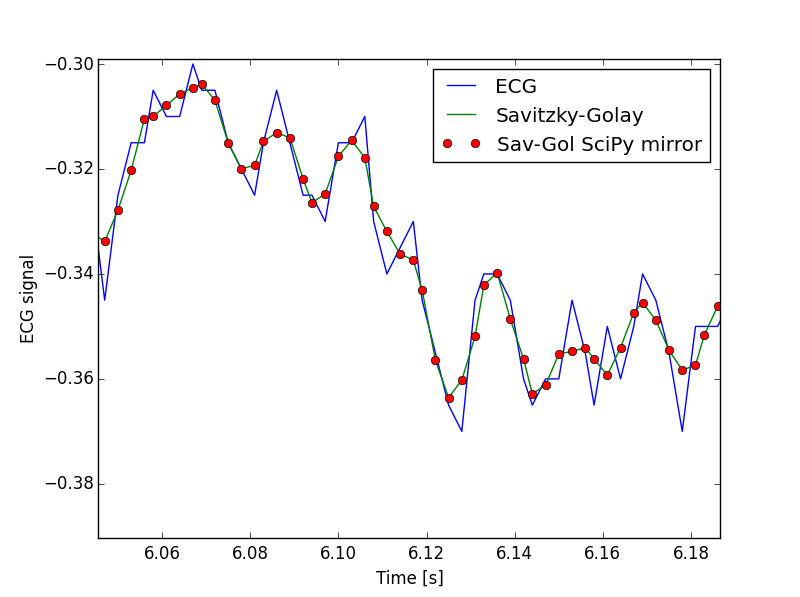
\includegraphics[scale=0.8]
    {img/prototype.png}
  \end{center}
  \caption{Wygładzanie metodą Savitzky-Golay z oknem 7 próbek (M=3) i aproksymacją wielomianem N=2 stopnia. Porównanie prototypu z funkcją z modułu SciPy.signals}
  \label{rys:savitzky_py}
\end{figure}

Aktualny kod dostępny w repozytorium https://github.com/Qbicz/Savitzky-Golay



\section{Implementacja}


Aktualny kod dostępny w repozytorium https://github.com/Qbicz/Savitzky-Golay

\bibliographystyle{IEEEtran}
\bibliography{bib/Bibliografia}

\end{document}

